\documentclass{article}
\linespread{0.7}
\usepackage[a4paper, margin=3mm, landscape]{geometry}
\usepackage{multicol}
\usepackage{xcolor}
\usepackage{enumitem}
\usepackage{amsmath}
\usepackage{amsfonts}
\usepackage{listings}
\usepackage{soul}
\usepackage{graphicx}

\pdfinfo{
    /Title (template.pdf)
    /Creator (TeX)
    /Producer (pdfTeX 1.40.0)
    /Author (securespider)
    /Subject (template)
    /Keywords (cheatsheet, pdf)
}

\graphicspath{ {./img/} }

\pagestyle{empty}
\setcounter{secnumdepth}{0}
\setlength{\columnseprule}{0.25pt}

% Redefine section commands to use less space
\makeatletter
\renewcommand{\section}{\@startsection{section}{1}{0mm}%
    {-1ex plus -.5ex minus -.2ex}%
    {0.5ex plus .2ex}%x
{\normalfont\large\bfseries}}
\renewcommand{\subsection}{\@startsection{subsection}{2}{0mm}%
    {-1explus -.5ex minus -.2ex}%
    {0.5ex plus .2ex}%
{\normalfont\normalsize\bfseries}}
\renewcommand{\subsubsection}{\@startsection{subsubsection}{3}{0mm}%
    {-1ex plus -.5ex minus -.2ex}%
    {1ex plus .2ex}%
{\normalfont\small\bfseries}}%
\makeatother

% Adjust spacing for all itemize/enumerate
\setlength{\leftmargini}{0.5cm}
\setlength{\leftmarginii}{0.5cm}
\setlist[itemize,1]{leftmargin=2mm,labelindent=1mm,labelsep=1mm}
\setlist[itemize,2]{leftmargin=2mm,labelindent=1mm,labelsep=1mm}

% Font
\renewcommand{\familydefault}{\sfdefault}

% Define colors for math formulas
\definecolor{myblue}{cmyk}{1,.72,0,.38}
\everymath\expandafter{\the\everymath \color{myblue}}

% Custom command for keywords
\definecolor{highlight}{RGB}{251,243,218}
\newcommand{\keyword}[2][]{\sethlcolor{highlight}\hl{\textbf{#2}} #1 - }
\newcommand{\ilkeyword}[1]{\sethlcolor{highlight}\hl{\textbf{#1}}}

% Define colors and style for code
\definecolor{codegreen}{rgb}{0,0.6,0}
\definecolor{codegray}{rgb}{0.5,0.5,0.5}
\definecolor{codered}{HTML}{CC241D}
\definecolor{backcolor}{rgb}{0.95,0.95,0.95}
\lstdefinestyle{codestyle}{
    backgroundcolor = \color{backcolor},
    commentstyle = \color{codegray},
    keywordstyle = \color{codered},
    stringstyle = \color{codegreen},
    basicstyle = \ttfamily,
    breakatwhitespace = false,
    showstringspaces = false,
    breaklines = true,
    showtabs = false,
    tabsize = 2
}
\lstset{style = codestyle}

% -----------------------------------------------------------------------
\begin{document}
\begin{multicols*}{3}
\footnotesize

% Title box
\begin{center}
    \fbox{
        \parbox{0.8\linewidth}{
            \centering \textcolor{black}{
                {\Large\textbf{CS3223}} \\
                \normalsize{[Database Systems Implementation]}} \\
                {\footnotesize \textcolor{gray}{github.com/securespider}}
        }
    }
\end{center}
\section{01. Storage}
DBMS stores:
\begin{itemize}
  \item Relations
  \begin{description}
    \item[Relation schemas]{Structure of relations, constraints, triggers}
    \item[View Definitions]
    \item[Indexes]{Derived information to speed up access to relations}
    \item{Statistical information about relations for use by query optimizer}
  \end{description}
  \item{Log files - Data recovery}
\end{itemize}

\begin{description}
  \item[Primary memory] Registers, static RAM (cache), dynamic RAM (physical mem)
  \item[Secondary memory]{Magnetic disk (HDD), solid-state disks}
  \item[Tertiary memory]{Optical disks, tapes}
  \item Tradeoff: Capacity, cost, access speed, volatility
\end{description}
\begin{itemize}
  \item DMBS stores data on non-volatile disk for persistence
  \item DBMS processes data in main memory
\end{itemize}
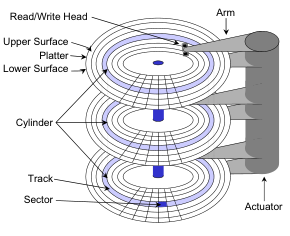
\includegraphics[scale=0.7]{hdd.png}
\begin{description}
  \item[Disk access time]
  \begin{description}
    \item[Command processing time] Interpreting access command by disk controller
    \item[Seek time]{Moving arms to position disk head on track ~5-6ms}
    \item[Rotational delay]{Waiting for block to rotate under head (~half revolution)}
    \item[Transfer time]{Actually moving data to/from disk surface (100-200microsecond)}
    \item Access time = seek time + rotational delay + transfer time
  \end{description}
\end{description}
SSD
\begin{itemize}
  \item NAND flash memory without moving parts
  \item Random: 100x Faster, Sequential: Slightly faster
  \item Lower power consumption
  \item Disadvantages:
  \begin{itemize}
    \item Update to a page requires erasure of multiple pages before overwriting page
    \item There is a limited number of times a page can be erased
  \end{itemize}
\end{itemize}
\subsubsection{Storage Manager Components} % (fold)
\label{ssub:storage_manager_components}
\begin{itemize}
  \item File \& access methods Manager
  \item Buffer pool manager
  \begin{itemize}
    \item Controls reading/writing of disk pages
  \end{itemize}
  \item Disk space manager
\end{itemize}

\subsubsection{Buffer Manager} % (fold)
\label{ssub:buffer_manager}


\begin{itemize}
  \item *Buffer pool* = main memory allocated for DBMS
  \item Partitioned into block-sized pages called frames
\end{itemize}
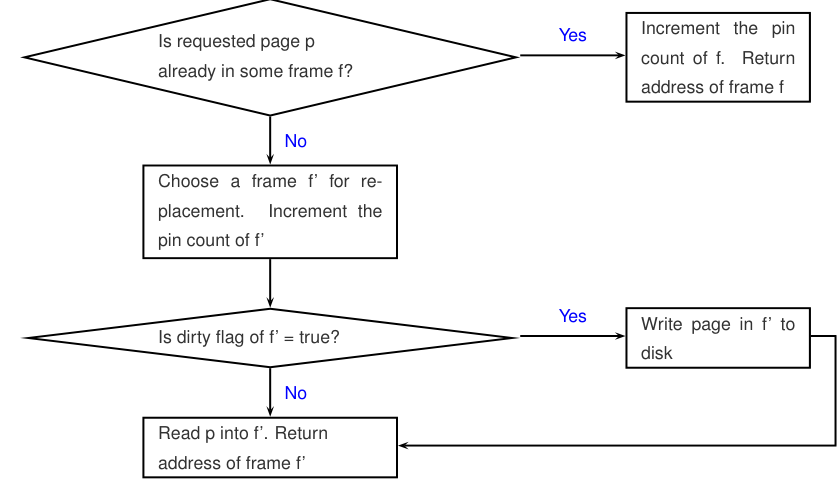
\includegraphics[scale=0.3]{buffermgmt.png}

Replacement policy
\begin{itemize}
  \item Random
  \item First in First Out
  \item Most Recently Used
  \item Least Recently Used
  \item Clock - current variable, referenced bit (replace page with referenced bit and pin out =0)
\end{itemize}
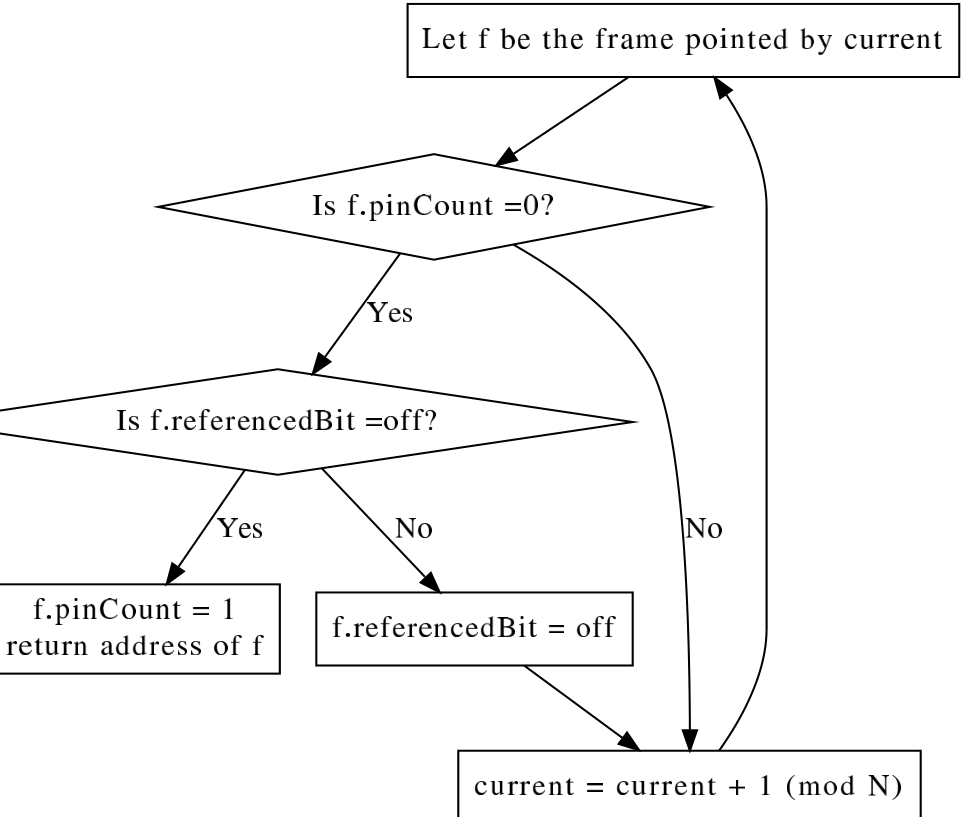
\includegraphics[scale=0.2]{clockreplacement.png}
% subsubsection buffer_manager (end)
% subsubsection storage_manager_components (end)

\subsubsection{Files} % (fold)
\label{ssub:files}

File abstraction: Operations
\begin{itemize}
  \item Create, delete, insert/delete/get records w RFID, scan
\end{itemize}

File Organisation = Arranging data records in a file that is stored on disk
\begin{itemize}
  \item Heap File: Unordered files
  \begin{itemize}
    \item Linked List Implementation: Header \-\>Data pages
    \item Page Directory Implementation w Fixed length records: RID = (page id, slot number)
  \end{itemize}
  \item Sorted File: Records ordered on search key
  \item Hashed file: Records in blocks via hash functions
\end{itemize}
% subsubsection files (end)
\subsubsection{Page Organisation} % (fold)
\label{ssub:page_organisation}

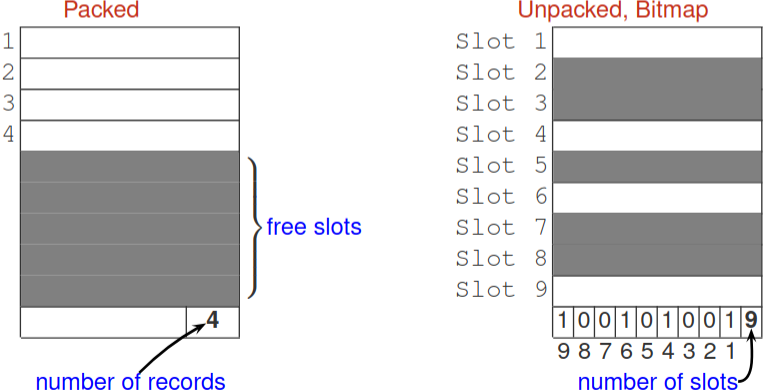
\includegraphics[scale=0.2]{fixed_length.png}
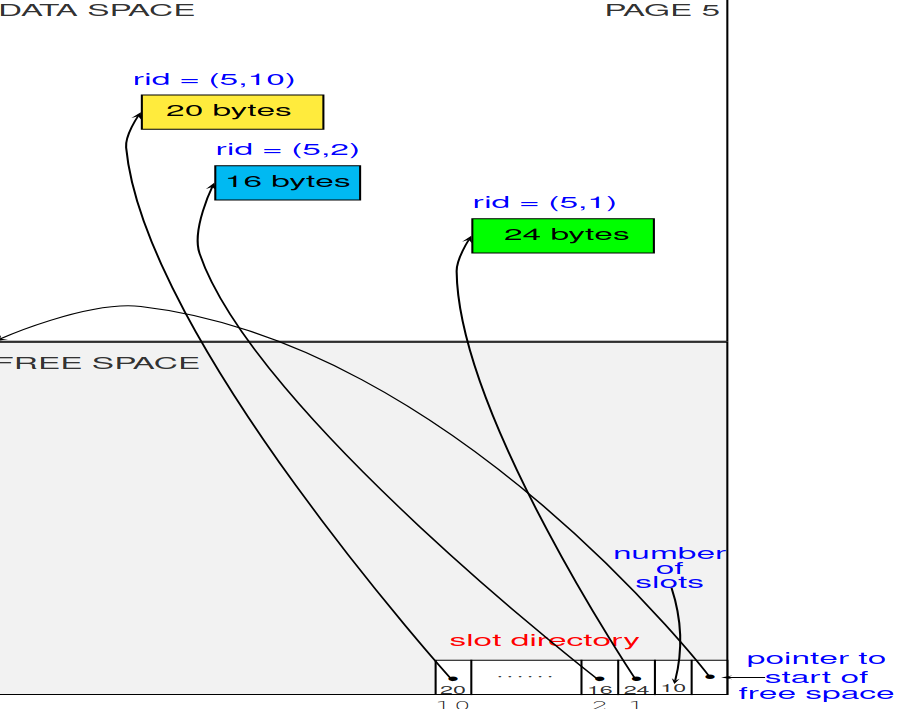
\includegraphics[scale=0.16]{variable_length.png}
\begin{itemize}
  \item Slotted page organisation splits pages into data vs free space
  \item RID references the position of pointer in the slot directory
  \item Maintaining RID means that the position of the pointer must be the same
\end{itemize}
\begin{description}
  \item[Forwarding record]{RID is unchanged where record is another pointer to the location of the data}
\end{description}
% subsubsection page_organisation (end)

\section{Lecture 2: B+ Tree Index} % (fold)
\label{sec:lecture_2_b+_tree_index}
\begin{description}
  \item[Index] Data structure to speed up retrieval of data records
  \item[Search key]{Sequence of k$\geq$ 1 data attributes}
  \begin{itemize}
    \item Composite search key if k $>$ 1
  \end{itemize}
  \item[Unique index]{Search key contains a candidate key of index table}
  \item[Tree-based index]{Based on sorting of search key values eg. ISAM, B+}
  \item[Hash-based index]{Data entries accessed using hashing eg. static, extendible, linear}
\end{description}
\subsubsection{B+ Tree} % (fold)
\label{ssub:b_tree}
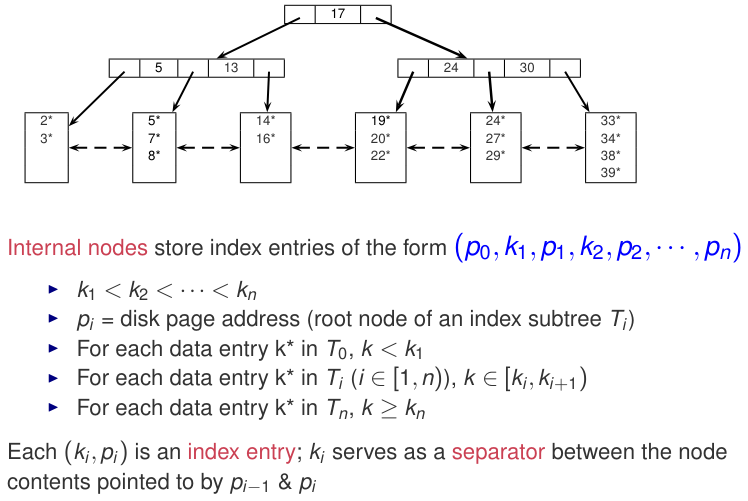
\includegraphics[scale=0.35]{b_tree.png}
\begin{description}
  \item[Order of index tree]{Controls space utilization}
  \begin{itemize}
    \item Non-root nodes contains m entries, where $m\in [d, 2d]$
    \item Root node contains m entries, where $m\in [1,2d]$
  \end{itemize}
\end{description}
Equality Search
\begin{itemize}
  \item At each internal node N, find largest key $k_i$ in N such that $k_i\leq k$
  \item If $k_i$ exists, search subtree at $p_i$
\end{itemize}

Formats of data entries
\begin{description}
  \item[Format 1]{Actual data record}
  \item[Format 2]{(k, rid) where rid is record identifier of data record}
  \item[Format 3]{(k, rid-list), format 2 but can point to multiple data records}
\end{description}

Insertion with splits
\\
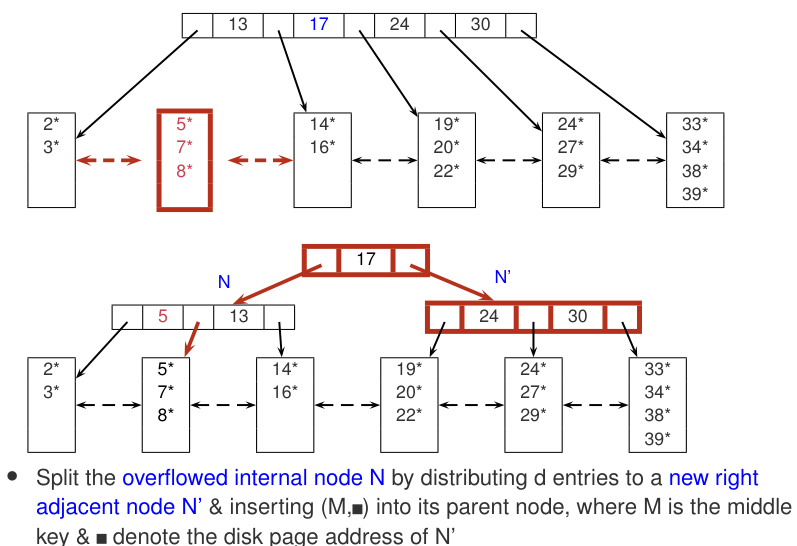
\includegraphics[scale=0.3]{tree_split.png}
\\
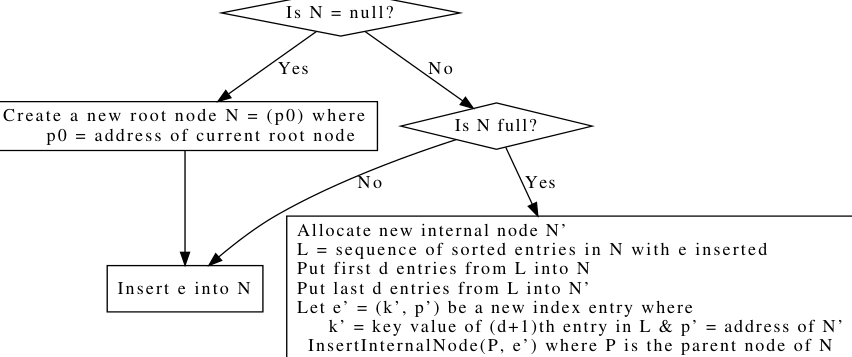
\includegraphics[scale=0.2]{tree_split_pseudo.png}
\begin{itemize}
  \item Split key goes to the right node (distribute d+1 entries to new leaf)
  \item Redistribution only checks right sibling then left sibling else node split
\end{itemize}

Deletion with merges
\\
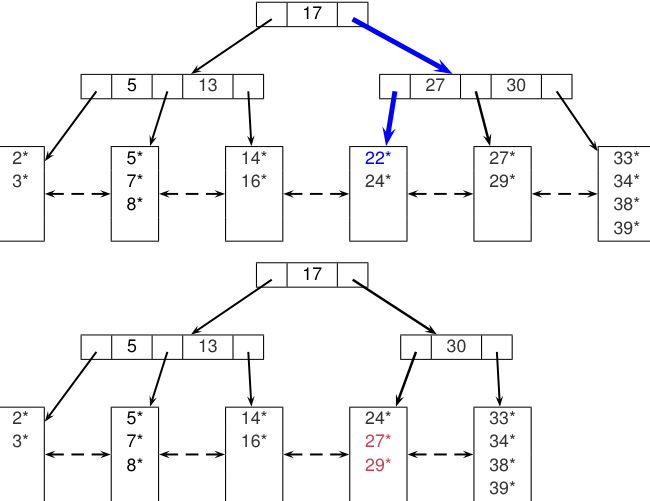
\includegraphics[scale=0.169]{tree_delete1.png}
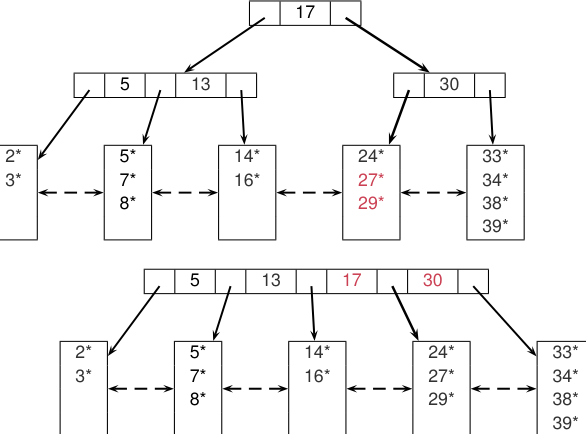
\includegraphics[scale=0.2]{tree_delete2.png}
\begin{itemize}
  \item Redistribute by taking from adjacent sibling node first
  \item Should only merge where adjacent sibling node has less than m entries
  \item Redistribution of internal entries attempted whenever possible
\end{itemize}
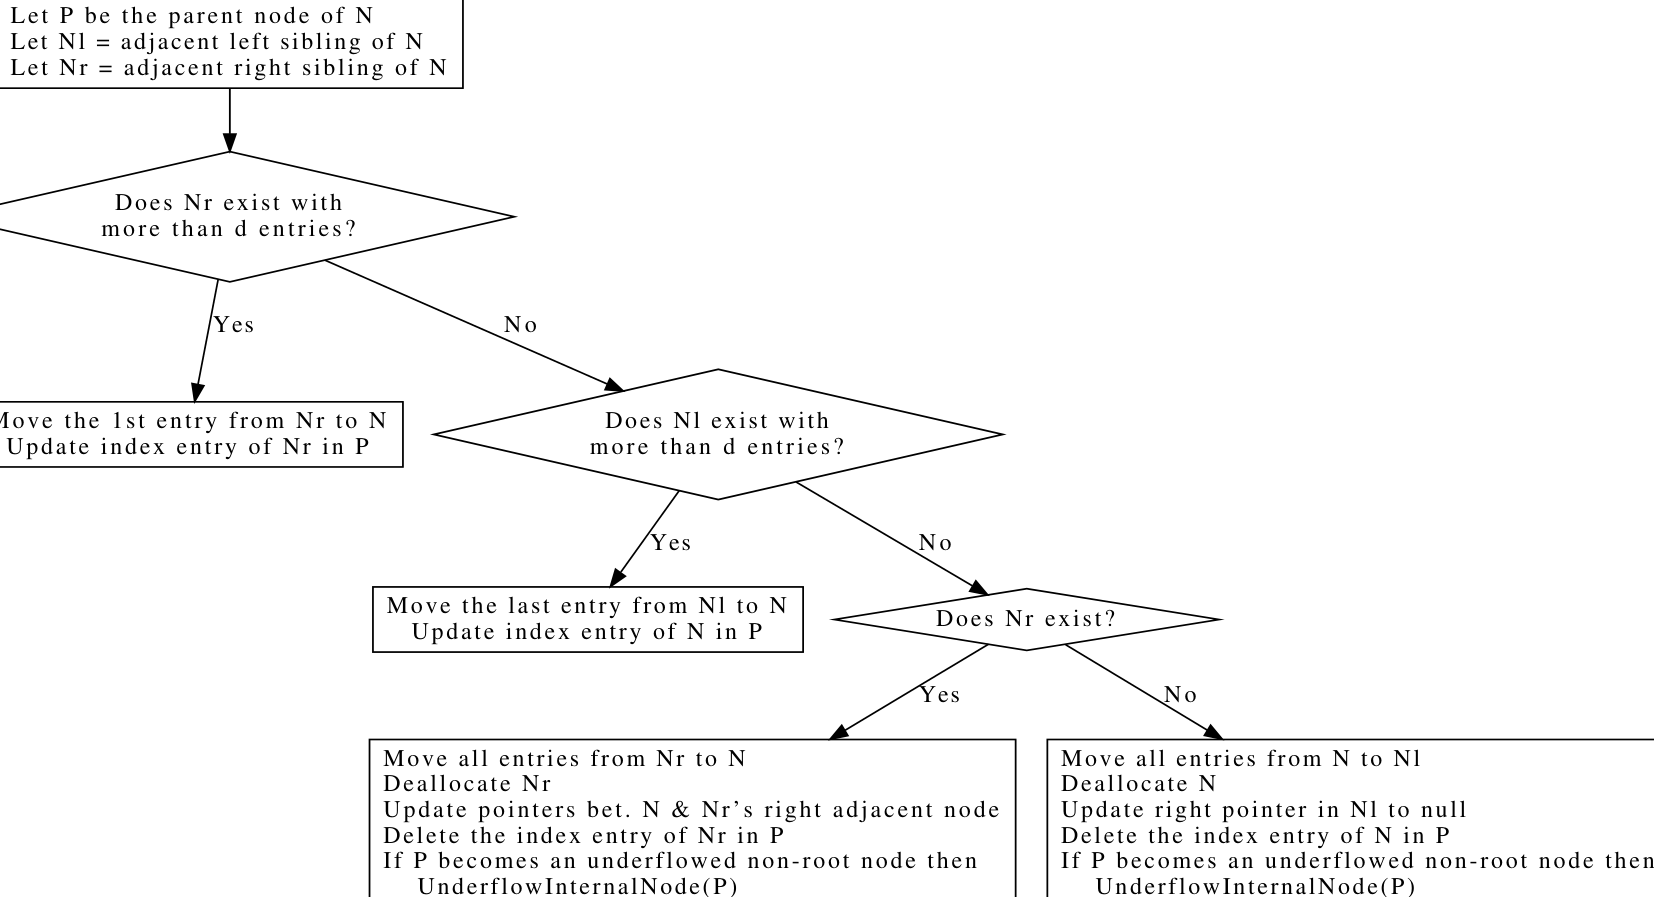
\includegraphics[scale=0.15]{tree_delete_pseudo.png}
\\
\begin{description}
  \item[Clustered index] Data is stored together with its RID
  \item[Unclustered index]{Relation is stored in a heap file referenced by this index}
\end{description}

Bulk loading of B+ Tree
\begin{itemize}
  \item Sort the indices and place them in 2*d buckets
  \item Take first number of each bucket as the separator of internal node
  \item Propagate internal node and parent nodes once the internal node has 2*d entries
\end{itemize}
% subsubsection b_tree (end)
% section lecture_2_b+_tree_index (end)

\subsection{Lecture 3: Hash-based Indexing} % (fold)
\label{sub:lecture_3_hash_based_indexing}



% subsection lecture_3_hash_based_indexing (end)






\end{multicols*}
\end{document}
